\begin{figure}[H]
	\centering
	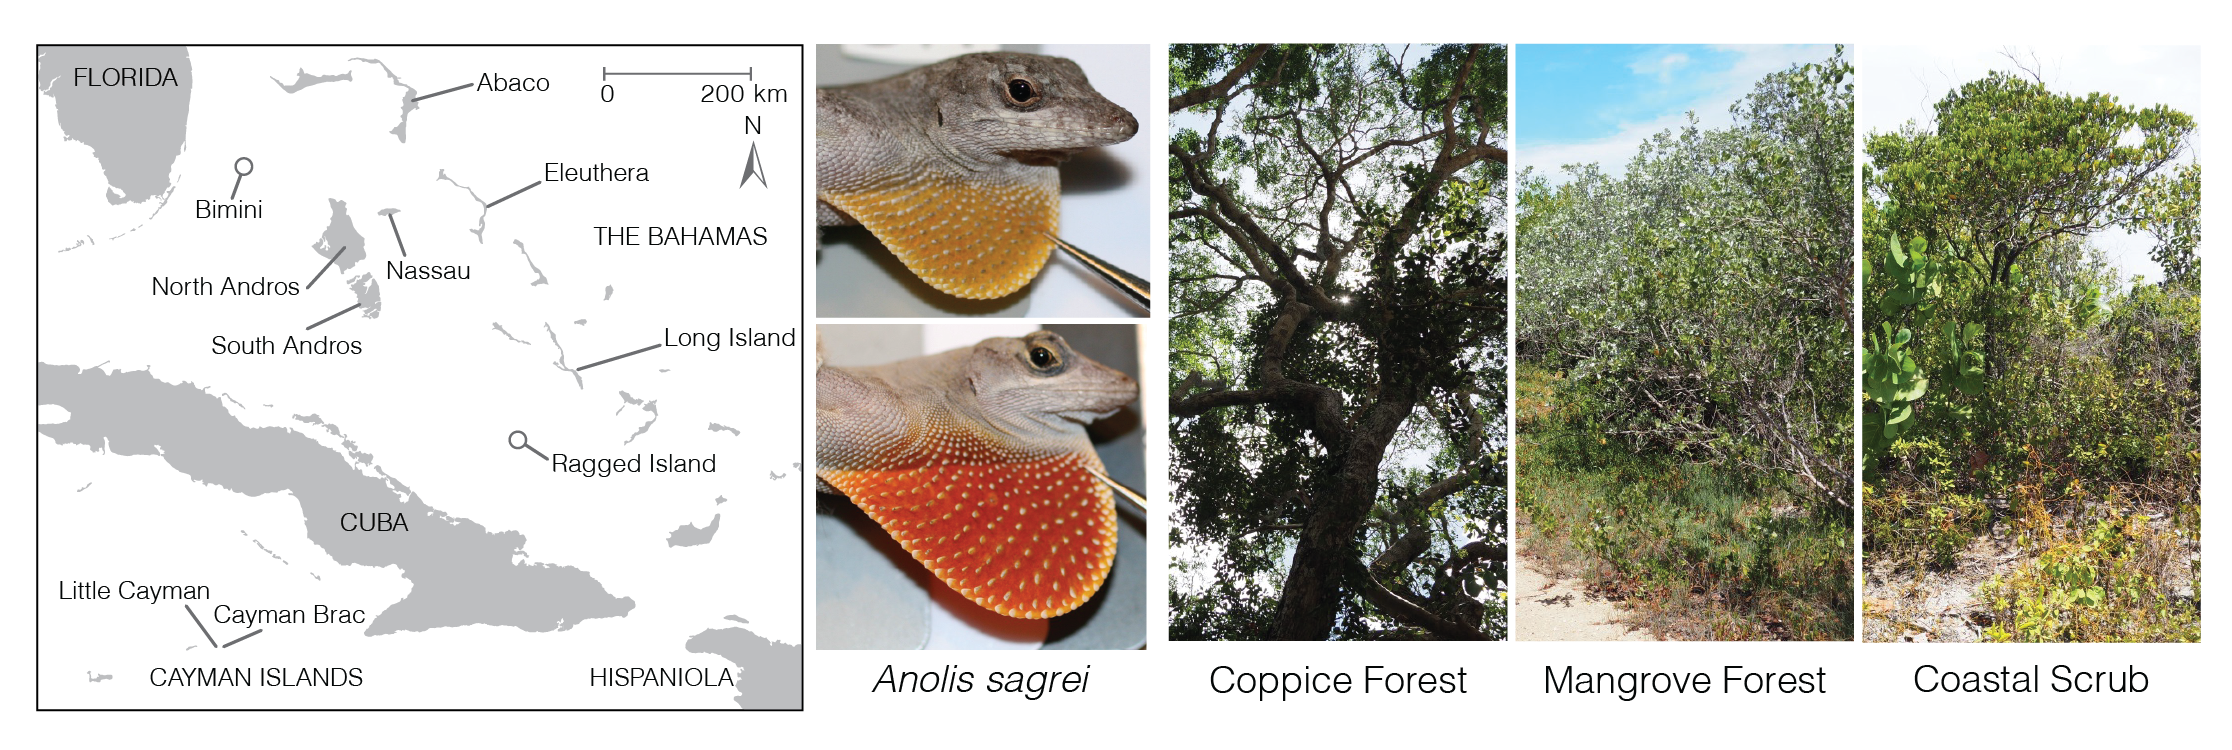
\includegraphics[width=\textwidth]{figures/Figure1_CMD-01_cropped.png}
	\caption{Overview of our study design, including a map of the Bahamas and the Cayman Islands, on which are indicated the nine islands we sampled, two representatives of our study species \textit{Anolis sagrei} with their dewlaps deployed, and the three types of habitats we considered on each island.}
	\label{fig:overview}
\end{figure}

\begin{figure}[H]
	\centering
	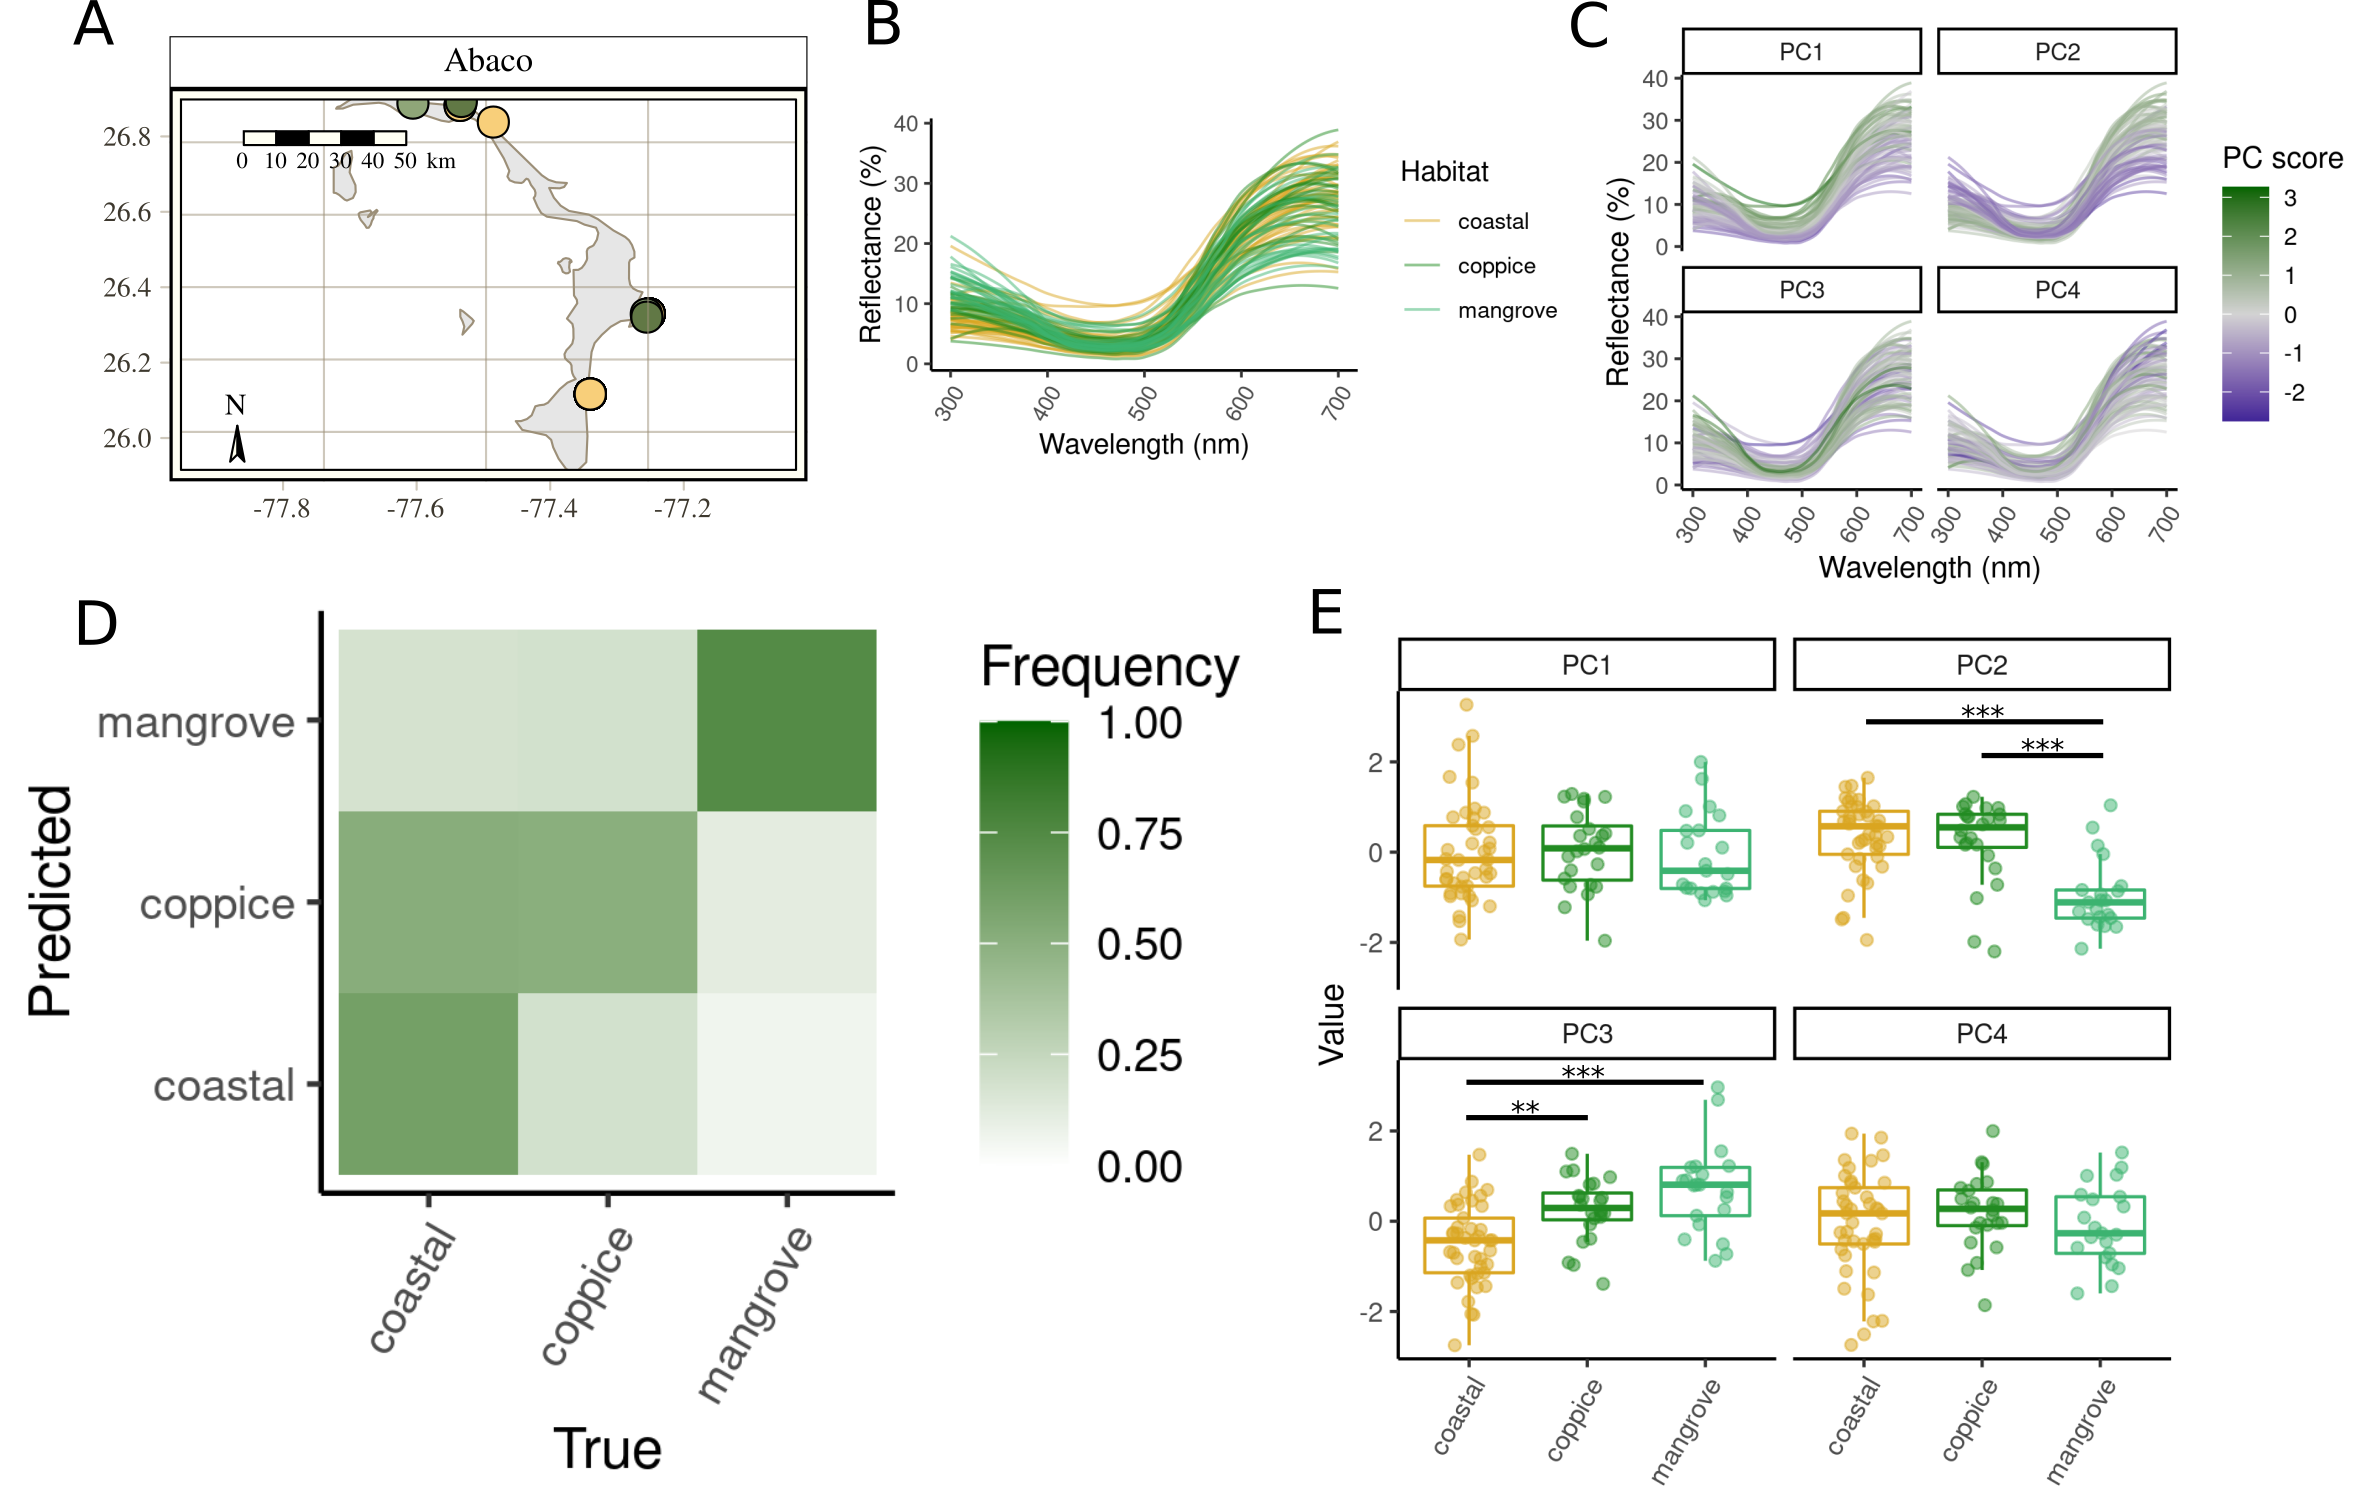
\includegraphics[width=\textwidth]{figures/Abaco_2.2.png}
	\caption{Comparison of dewlap coloration across habitats on Abaco. (A) Map of the island with the sampling sites colored by habitat. (B) Reflectance profiles of all the dewlaps on the island. (C) How reflectance profiles map onto the within-island principal components. (D) Confusion matrix showing the proportion of lizards from each (true) habitat reassigned to each (predicted) habitat by the random forests, based on the first four within-island principal components and averaged across replicates. Each column sums to one. (E) Within-island principal component scores across habitats. Bars indicate significant contrasts. *, $P < 0.05$; **, $P < 0.01$; ***, $P < 0.001$.}
	\label{fig:Abaco}
\end{figure}